% This file is modified by Frans Oliehoek <faolieho@science.uva.nl>
% on 2005/12/18. (original file name: conference-ornate-20min.en.tex)

\documentclass[11pt]{beamer}

% Copyright 2004 by Till Tantau <tantau@users.sourceforge.net>.
%
% In principle, this file can be redistributed and/or modified under
% the terms of the GNU Public License, version 2.
%
% However, this file is supposed to be a template to be modified
% for your own needs. For this reason, if you use this file as a
% template and not specifically distribute it as part of a another
% package/program, I grant the extra permission to freely copy and
% modify this file as you see fit and even to delete this copyright
% notice. 

\mode<presentation>
{
\usetheme{IAS_topNav_bottomAuthorTitle}
  \setbeamercovered{transparent}
}
\setbeamertemplate{navigation symbols}{} % to remove the navigation symbols:

%%%%%%% PACKAGES
\usepackage[english]{babel}
\usepackage[latin1]{inputenc}
\usepackage{times}
\usepackage[T1]{fontenc}
\usepackage{wrapfig}


%%%%%%% PROPTERTIES
\title{Naxsi performance measurement}
\subtitle{Performance of a whitelist WAF}
\author{Lutz Engels \and Dennis Pellikaan}
\institute[University of Amsterdam] % (optional, but mostly needed)
{
{\large University of Amsterdam} \\
System and Network Engineering
}
\date{March 26, 2013}
\pgfdeclareimage[height=0.5cm]{institution-logo}{uva_logo}
\logo{\pgfuseimage{institution-logo}}


%%%%%%%%%%%%%%%%%%%%%%%%%%%%%%%%%%%%%%%%%%%%%%%%%%%%%%%%%%%%%%%%%%%%%%%%%%%%%%%%%%%%%%


%%%%%%% CONTENT
\begin{document}

%%%%%%% TITLE-PAGE
\begin{frame}
  \titlepage
\end{frame}


\begin{frame}
  \frametitle{Outline}
  \tableofcontents
\end{frame}

%%%%%%% CONTENT SPLIT UP IN TWO
\section{Naxsi}

%%%%%%% SECTION 1/3
\begin{frame}
  \frametitle{What is a WAF?}
   \begin{itemize}
   \item Web Application Firewall 
   \item 
  \end{itemize}
\end{frame}

\begin{frame}
  \frametitle{What is a naxsi?}
   \begin{itemize}
   \item It's a WAF for nginx
   \item Nginx Anti Xss \& Sql Injection
   \item designed as reverse proxy
  \end{itemize}
\end{frame}

\begin{frame}
  \frametitle{Naxsi request flow}
\begin{tabular}{ll}
\begin{minipage}[c]{0.3\textwidth}
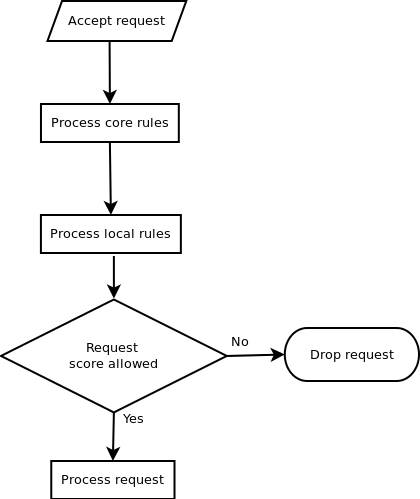
\includegraphics[width=\textwidth]{../paper/images/naxsi_flow.png}
\end{minipage}
&
\begin{minipage}[c]{0.7\textwidth}
  \begin{itemize}
   \item Oui!
   \item Sis is mooi sjrafiek
  \end{itemize}
\end{minipage}
\end{tabular}
\end{frame}


\begin{frame}
  \frametitle{Whitelist processing}
   \begin{itemize}
   \item 
   \item 
   \item
  \end{itemize}
\end{frame}


\begin{frame}
  \frametitle{Experimental setup}
    \begin{center} 
      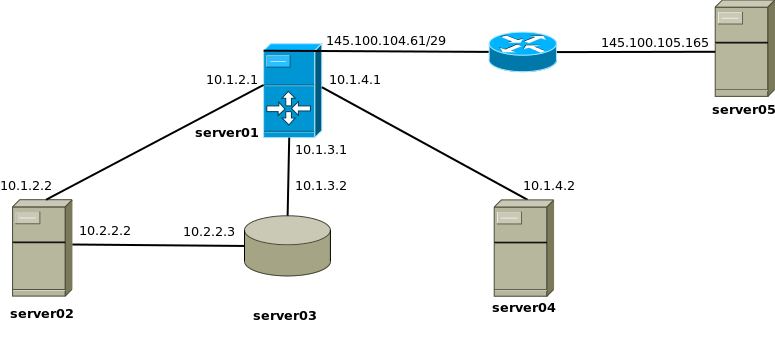
\includegraphics[width=0.80\textwidth]{../paper/images/infrastructure.png}
  \end{center}
\end{frame}


\begin{frame}
  \frametitle{Research Question(s)}
   \begin{center}
   \LARGE{"How does a webserver perform with the use of Naxsi as the front-end firewall
compared to a webserver without a Naxsi firewall?"}\\OR\\
   \LARGE{"How does the use of Naxsi as the front-end firewall influence the performance of a webserver?"}
  \end{center}
\end{frame}

\begin{frame}
  \frametitle{Research Question(s)}
   \begin{center}
   \LARGE{"What is the baseline performance of the Nginx firewall without the usage of Naxsi?"}
  \end{center}
\end{frame}


\section{Research questions}

%\section{Future work}

%%%%%%% QUESTIONS
\begin{frame}[noframenumbering]
  \frametitle<presentation>{References}
  \begin{itemize}
   \item naxsi: \\ \url{https://code.google.com/p/naxsi/}
   \item NaxsiBench: \\ \url{https://code.google.com/p/naxsi/wiki/NaxsiBench}
  \end{itemize}
\end{frame}


\end{document}
